\chapter{Resource Access Protocols}
\section{Introduction}
A \side{resource} is any software structure that can be used by a process to advance its executino. Tipically,  a resource can be a data structure, a set of variables, a main mamory area, a file, or a set of registers of a peripheral device. A resource dedicated to a particular process is said to be \textit{private}, whereas a resource that can be used by more tasks is called a \textit{shared resource}. A shared resource protexted against concurrent accesses is called an \textit{exclusive resource}.

To ensure consistency of the data structures in exclusive resources, any concurrent operating system should use appropriate resource access protocols to guarantee a mutual exclusion among competing tasks. A piece of code executed under mutual exclusion contraints is called a \side{critical section}.

Any task that needs to enter a critical section must wait until no other task is holding the resource. A task waiting for exclusive resource is said to be \textit{blocked} on that resource, othertwise it proceeds by entering the critical section and holds the resource. When a task leaves a critical section, the resource associated with the critical section becomes \textit{free}, and it can be allocated to another waiting task, if any.

In this chapter, we describe the main problems that may arise in a uniprocessor system when concurrent tasks use shared resources in exclusive mode, and we present some resource access protocols designed to avoid such problems and bound the maximum blocking time of each task. We then show how such blocking times can be used in the schedulability analysis to extend the guaranteee tests derived for periodic task sets.

\subsection{Atomicity}
So far we have assumed that all tasks that run and compete for a processor are independent, which means that they do not interact with one another. But there are several occasions in which this assumption cannot be made (e.g. when two tasks need to share information, exchange variables,\dots).
The other is when you have to compete for shared resources.

In this section we will introduce this problem and in particular we will introduce the notion of atomicity.
\definition{Atomic Instruction}{An atomic instruction is an instruction whose execution cannot be interleaved with the execution of other instructions}
In this sense atomic operations are always sequentialized since they cannot be interrupted. Under these conditions they are safe operations.\\
On the other hand, non atomic operations can be interrupted, and as such they are not \textit{safe} operations.

Usually, it is preferrable to have, whenever possible, non atomic operations, because they allow you to exploit in full the possibility of scheduling the processor to activities having higher priority via preemption.

\example{Non atomic operations}{
    Conside a simple operation like 
    \[x = x+1\]
    The variable is stored in a memory address that we call $x$. Hence, whenever the variable is incremented using this operation, we would have to:
    \begin{itemize}
        \item load the variable $x$ into a register $R0$
        \begin{center}
        \texttt{LD  R0, x}
        \end{center}
        \item increment the register
        \begin{center}
            \texttt{INC  R0}
        \end{center}
        \item store back the value contained in the register into $x$
        \begin{center}
        \texttt{ST  x, R0}
        \end{center}
    \end{itemize}
}
If the same operation is executed inside an interrupt handler an inconsistency may arise.

\example{Interrupt on non-atomic operations}{
Let us consider that the increment operation is both applied in the normal code and in an interrupt handler code (routine executed in response to an interrupt).\\
In both cases, the operation is translated into the assembly language using three instructions (load, increment and store).

The program starts executing as follows:
\begin{enumerate}
    \item The normal code starts executing: the value of $x$ is loaded from memory to the register
    \item At some point during this operation something triggers the execution of the interrupt
    \item The interrupt handler creates a copy of all the registers
    \item The interrupt handler load (once again) $x$ from memory, increments the register and stores the result in memory (the value of $x$ in memory has changed to $x+1$)
    \item Upon the interrupt handler has completed, the saved registers are restored. Hence, the old value of the register (i.e. $x$) is loaded back, its value is incremented to $x+1$ and stored into memory at the address of $x$ 
\end{enumerate}
The problem is that even though the code should have performed two increments (i.e. the final value should have been $x+2$), it yields the incorrect result (i.e. $x+1$).

From a logical point of view two increment operations should have taken place, but in effect one of them not successfully completed because while i was incrementing the variable, I was allowed to be interrupted and I was left with a state that was not up to date.
}

The nasty problem about this phenomenon is that it does not always happen in this way, because sometimes the function successfully completes before the interrupt is fired.\\
The example provided is the description of a condition called \side{critical race}, because you can have multiple execution of your code that interleave the operation in slightly different ways and you obtain different results.

This is a nasty problem in computer science because it might not materialize for years.

This is so because you cannot make assumption about the speed of the hardware and on the exact moment when certain events take place (we do not know the order of execution of the hardware instructions).

The case studies proposed are a perfect example of a not atomic operation that should be atomic.

The same behaviour occurs not only in the case of interrupts but also on interleaving tasks: so you could have two tasks running in parallel, both of which are sharing the variable $x$.

We can give a few definitions that are important for the follow up of our discussion:
\definition{Shared Object}{An object where the conflict may happen.}
\definition{Critical section}{A critical section is a sequence of operations that cannot be interleaved with other operations on the same resource}
\definition{Mutual exclusion}{Two critical sections cannot be active at the same time (they must be sequentialized). Either one or the other needs to stand by while the other executes}

There are three ways to obstain mutual exclusion:
\begin{enumerate}
    \item Implementing the critical section as an atomic operation.\\
    This that interrupt are disabled before the execution of the critical section and then are restored upon termination of the operation. The problem with this is that it is really tough because disabling the interrupts the I/O system of the machine is no longer allowed to work properly. (pressing an emergency button will have no effect and the execution of the code will continue),\\
    Moreover if the critical section is long, no interrupt can arrive during the critical section. In the case of a timer interrupt that arrives every 1ms, if a critical section lasts more than 1ms, a timer interrupt could be lost!
    \item Disabling the preemption (system-wide).\\
    This strategy will have some problems, because all the tasks will suffer from this suspention of the preemption even though they do not use shared resources.
    \item Selectively disabling the preemption (using semaphores and mutual exclusion).\\
    This strategy will disable preemption only for the task that operates on the shared resource.
\end{enumerate}
Hence, we should try to disable preemption rather than disabling interrupts.

Still the big issue with selectively disabling preemption the priority mechanism is no longer enforced: during the critical section might force the process to execute low priority tasks because preemption is disabled. This phenomenon is known as \side{Priority Inversion}.

If Priority inversion is not correctly managed it may lead to a complete violation of all timing contraints.
\subsection{Interacting Tasks}
Until now, we have considered only independent tasks, which are characterized by the fact that a job never blocks or suspends and a task only blocks on job termination.\\
In the real world, jobs might block for various reasons:
\begin{itemize}
    \item Tasks exchange data throught shared memory (mutual exclusion)
    \item A task might need to synchronize with other tasks while waiting for some data
    \item A job might need a hardware resource which is currently not available.
\end{itemize}

\example{Control Application}{
    Let us consider a control application composed by three periodic tasks:
    \begin{itemize}
        \item $\tau_1$ reads the data from the sensors and applies a filter. The results are stored in memory.
        \item $\tau_2$ reads the filtered data and computes some control law (updating the state and the outputs); both the state and the outputs are stored in memory
        \item $\tau_3$ reads the outputs and writes on an actuator
    \end{itemize}
    All of the three tasks access data in shared memory. This means that there are conflicts on accessing this data concurrently with the risk that the data structures become inconsistent.
    }

\subsection{Priority Inversion Phenomenon}

The rest of this chapter presents the following resource access protocols:
\begin{itemize}
    \item Non-Preemptive Protocol (NPP)
    \item Highest Locking Priority (HLP)
    \item Priority Inheritance Protocol (PIP)
    \item Priority Ceiling Protocol (PCP)
\end{itemize}

\section{Non Preemptive Protocol (NPP)} 
A simple solution that avoids the unbounded priority inversion problem is to disallow preemption during the execution of any critical section. This method, also referred to as \side{Non-Preemptive Protocol (NPP)}, can be implemented by raising the priority of a task to the highest priority level whenever it enters a shared resource. In particular, as soon as a task $\tau_i$ enters a resource $R_k$, its synamic priority is raised to the level:
\[p_i(R_k) = \max_h \{p_h\}\]
The dynamic priority is then reset to the nominal value $p_i$ when the task exits the critical section.

\begin{figure}[!h]
    \centering
    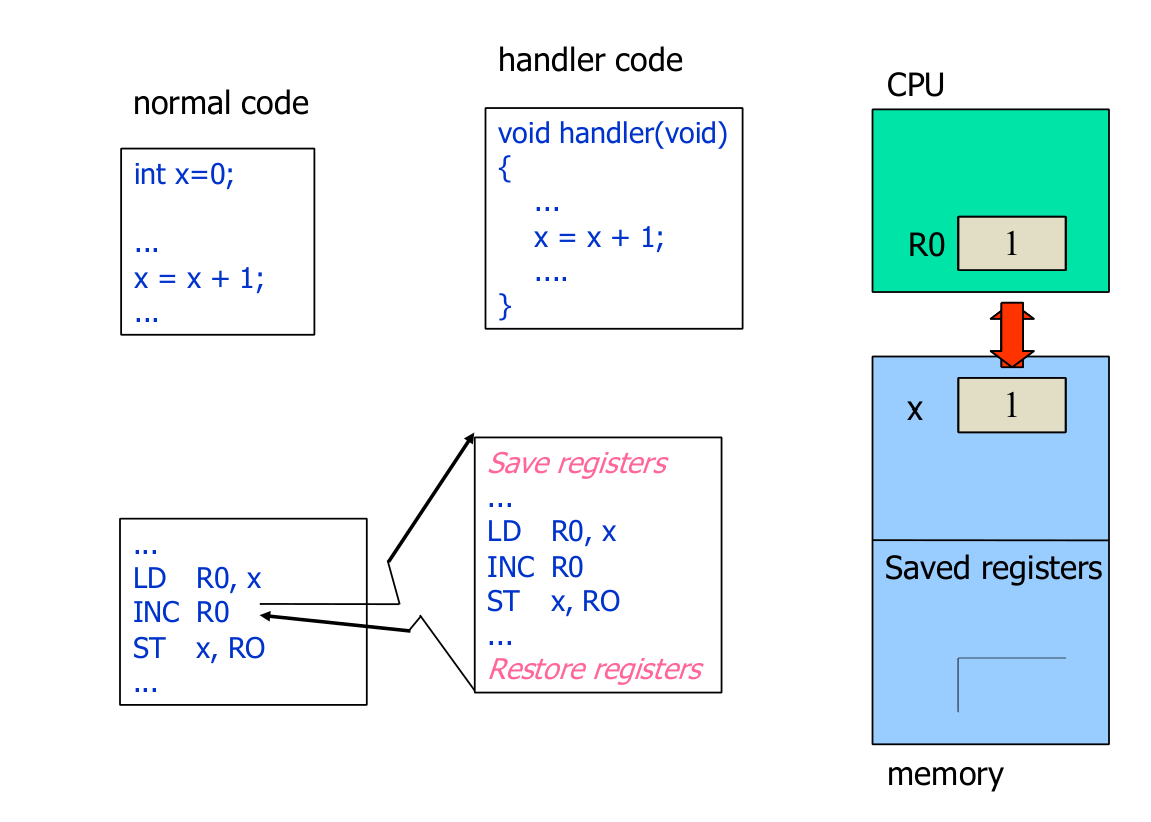
\includegraphics[width =0.75\textwidth]{images/image06.png}
\end{figure}


This method solves the priority inversion phenomenon, however, is only appriopriate when tasks use short critical sections because it creates unnecessary blocking. This actually might cause deadline misses of tasks that do not use the shared resource.

\begin{figure}[!h]
    \centering
    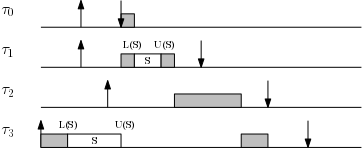
\includegraphics[width =0.75\textwidth]{images/image07.png}
\end{figure}
In the example, $\tau_0$ misses its deadline (suffers a blocking time equal to 3) even though it does not use any resource!!\\
The solution is to raise $\tau_3$ priority to the maximum between tasks accessing the shared resource (i.e. $\tau_1$) priority.



\section{Highest Locking Priority (HLP)}
The \side{Highest Locking Priority (HLP)} protocol improves NPP by raising the priority of a task that enters a resource $R_k$ to the highest priority among the tasks sharing that resource. In particular as soon as a task $\tau_i$ enters a resource $R_k$, its dynamic priority is raised to the level
\begin{equation}
\label{eq:equation2}
p_i(R_k) = \max_h\{p_i | \tau_h \text{ uses } R_k\}
\end{equation}

The dynamic priority is then reset to the nominal value $p_i$ when the task exits the critical section. The online computation of the priority level in equation \ref{eq:equation2} can be simplified by assigning each resource $R_k$ a \side{priority ceiling} $C(R_k)$ (computed offline) equal to the maximum priority of the tasks sharing $R_k$; that is:
\[C(R_k) = \max_h\{p_i | \tau_h \text{ uses } R_k\}\]
Then, as soon as a task $\tau_i$ enters a resource $R_k$, its dynamic priority is raised to the ceiling of the resource. For this reason, this protocol is also referred to as \side{Immediate Priority Ceiling}.

\begin{figure}[!h]
    \centering
    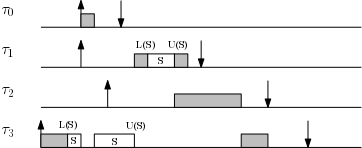
\includegraphics[width =0.75\textwidth]{images/image08.png}
\end{figure}

\section{Priority Inheritance Protocol (PIP)}
The \side{Priority Inheritance Protocol (PIP)} proposed by Sha, Rajkumar and Lehoczky, avoids unbounded priority inversion by modifying the priority of those tasks that cause blocking. In particular, when a task $\tau_i$ blocks one or more higher-priority tasks, it temporarily assumes (\textit{inherits}) the highest priority of the blocked tasks. This prevents medium-priority tasks from preempting $\tau_i$ and prolonging the blocking duration experienced by the higher-priority tasks.

The Priority Inheritance Protocol can be defined as follow:
\begin{itemize}
    \item Tasks are scheduled based on their active priorities. Tasks with the same priority are executed in a First Come First Served discipline.
    \item When task $\tau_i$ tries to enter a critical section and resource $R_k$ is already held by a lower-priority task $\tau_j$, then $\tau_i$ is blocked. $\tau_i$ is said to be blocked by the task $\tau_j$ that holds the resource. Otherwise, $\tau_i$ enters the critical section.
    \item When a task $\tau_i$ is blocked, it transmits its active priority to the task $\tau_j$ that holds the semaphore/mutex. Hence, $\tau_j$ resumes adn executes the rest of its critical section with a priority $p_j = p_i$. Task $\tau_j$ is said to inherit the priority of $\tau_i$. In general, a task inherits the highest priority of the tasks it blocks. That is, at every instant,
    \begin{equation}
        \label{eq:equation3}
        p_j(R_k) = \max \{P_j, \max_h \{P_h | \tau_h \text{ is blocked on }R_k\}\}
    \end{equation}
    \item When $\tau_j$ exits a critical section, it unlocks the mutex/semaphore, and the highest-priority task blocked, if any, is awakened. Moreover, the avtive priority of $\tau_j$ is updated as follows: if no other tasks are blocked by $\tau_j$, $p_j$ is set to its nominal priority $P_j$; otherise it is set to the highest priority of the tasks blocked by $\tau_j$, according to equation \ref{eq:equation3}.
    \item Priority inheritance is transitive; that is, if a task $\tau_3$ blocks a task $\tau_2$, and $\tau_2$ blocks a task $\tau_1$, then $\tau_3$ inherits the priority of $\tau_1$ via $\tau_2$
\end{itemize}

A high priority task can experience two kinds of blocking: \side{Direct blocking} and \side{Push-through blocking}.


\definition{Direct blocking}{It occurs when a higher-priority task tries to acquire a resource already held by a lower-priority task. Direct blocking is necessary to ensure the consistency of the shared resources}
\definition{Push-through blocking}{It occurs when a medium-priority task is blocked by a low-priority task that has inherited a higher priority from a task it directly blocks. Push-through blocking is necessary to avoid unbounder priority inversion}


\begin{figure}[!h]
    \centering
    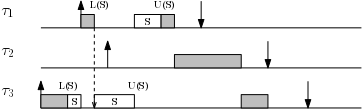
\includegraphics[width =0.75\textwidth]{images/image09.png}
\end{figure}

Although the Priority Inheritance Protocol bounds the priority inversion phenomenon, the blocking duration for a task can still be substantial because a chain of blocking can be formed. Another problem is that protocol does not prevent deadlocks (however, the latter problem can be solved by imposing a total ordering on the mutex accesses).

\section{Priority Ceiling Protocol (PCP)} % follow lecture
The \side{Priority Ceiling Protocol (PCP)} was introduced by Sha, Rajkumar, and Lehoczky to bound the priority inversion phenomenon and prevent the formation of deadlocks and chained blocking.

The basic idead of this method is to extend the Priority Inheritance Protocol with a rule granting a lock request on a free mutex. To avoid multiple blocking, this rule does not allow a task to enter a critical seciton if there are locked mutexes that could block it. This means that once a task enters its first critical section, it can never be blocked by lower-priority tasks until its completion.

In order to realize this idea, each mutex is assigned a priority ceiling equal to the highest priority of the tasks that can lock it. Then, a task $\tau_i$ is allowed to enter a critical section only if its priority is higher than all priority ceiling of the mutexes currently locked by tasks other than $\tau_i$.
\subsection{Original Priority Ceiling Protocol (OPCP)}

The \side{Original Priority Ceiling Protocol} can be defined as follows:

\subsection{Immediate Priority Ceiling Protocol (IPCP)}